\documentclass[journal]{IEEEtran}

\usepackage{cite,stfloats,url}
\usepackage{amsmath,amsfonts,amssymb,amscd}
\usepackage[caption=false,font=footnotesize]{subfig}
\usepackage{float,color,xcolor, pgfplots, ifthen, multirow,soul,tikz} %xcolor
\pdfsuppresswarningpagegroup=1

\newcommand*{\mycheckmark}[1][]{\tikz[x=1em, y=1em]\fill[#1] (0,.35) -- (.25,0) -- (1,.7) -- (.25,.15) -- cycle;}

% for Jingwei's crazy table
\usepackage{multirow}
%\usepackage[table,xcdraw]{xcolor}
%\usepackage{colortbl} % for \rowcolor
%\definecolor{Grayy}{gray}{0.85}

% Do not include svg, and save as pdf instead.
%\usepackage{svg} %for \includesvg

\usepackage{arydshln} %for \hdashline
% Another combination of values % https://tex.stackexchange.com/questions/169098/dotted-line-instead-of-hline-in-table-environment
%\setlength\dashlinedash{0.2pt}
%\setlength\dashlinegap{1.5pt}
%\setlength\arrayrulewidth{0.3pt}

\usepackage{anyfontsize} % https://tex.stackexchange.com/questions/58087/how-to-remove-the-warnings-font-shape-ot1-cmss-m-n-in-size-4-not-available

%\pgfplotsset{compat=newest}
%\usepackage{tikz}
%\usepackage[american,cuteinductors,smartlabels]{circuitikz}
%\usetikzlibrary{intersections}
%\usetikzlibrary{calc}
%\usetikzlibrary{backgrounds,positioning}

% for using new line in table
%\usepackage{makecell}
%\renewcommand\theadalign{bc}
%\renewcommand\theadfont{\bfseries}
%\renewcommand\theadgape{\Gape[4pt]}
%\renewcommand\cellgape{\Gape[4pt]}

% For Revision
%\usepackage[final]{changes} % it clears the traces of changes made by the authors and respecting the last changes.
%\usepackage[markup=underlined]{changes}
%\definechangesauthor[name={Jiahao Chen}, color=blue]{CJH}
%\definechangesauthor[name={Eric Loren Severson}, color=orange]{ELS}

% Simple Revision
 \definecolor{darkgreenOri}{RGB}{84, 139, 34}
 \definecolor{sthlmRedOri}{RGB}{196,0,100}
 \definecolor{ranewRedOri}{RGB}{220,0,120}
 \definecolor{darkBlueOri}{RGB}{15,40,127}
 \definecolor{sthlmBlueOri}{RGB}{0,110,191}
\newcommand{\idraft}[1]{#1} %{\textcolor{darkgreen}{#1}}
\newcommand{\ra}[1]{\textcolor{sthlmRedOri}{#1}}
\newcommand{\ranew}[1]{\textcolor{ranewRed}{#1}}
\newcommand{\ecce}[1]{#1} %{\textcolor{darkBlue}{#1}}
\newcommand{\rb}[1]{\textcolor{sthlmBlue}{#1}}

% Todo Notes
%\usepackage[colorinlistoftodos,prependcaption,textsize=small]{todonotes}
%%\usepackage[disable]{todonotes}
%\newcommand{\todoINFO}[1]{\todo[inline, color=blue!25]{INFO: #1}}
%\newcommand{\todoIMPORTANT}[1]{\todo[inline, color=red!25]{IMPORTANT: #1}}
%\newcommand{\todoREVA}[1]{\todo[inline, color=green!25]{REVISED: #1}}


% 转置符号不是T
\newcommand{\transpose}{^\mathsf{T}}
%$\mathbf{A}^\mathrm{T}$
%$\mathbf{A}^\top$
%$\mathbf{A}^\mathsf{T}$
%$\mathbf{A}^\intercal$

% 求导符号要正体
\newcommand{\derivative}{\frac{\mathrm{d}}{\mathrm{d}t}}

%评注结束符
\newcommand\xqed[1]{%
  \leavevmode\unskip\penalty9999 \hbox{}\nobreak\hfill
  \quad\hbox{#1}}
\newcommand\myendremark{\xqed{$\triangle$}}
% see https://tex.stackexchange.com/questions/16453/denoting-the-end-of-example-remark

\usepackage{siunitx} % Number only: \num{1e-10}

% Place text anywhere you like
\usepackage[pscoord]{eso-pic}% The zero point of the coordinate systemis the lower left corner of the page (the default).
\newcommand{\placetextbox}[3]{% \placetextbox{<horizontal pos>}{<vertical pos>}{<stuff>}
  \setbox0=\hbox{#3}% Put <stuff> in a box
  \AddToShipoutPictureFG*{% Add <stuff> to current page foreground
    \put(\LenToUnit{#1\paperwidth},\LenToUnit{#2\paperheight}){\vtop{{\null}\makebox[0pt][c]{#3}}}%
  }%
}%

% thank note as footnote
%\newcommand\blfootnote[1]{%
%  \begingroup
%  \renewcommand\thefootnote{}\footnote{#1}%
%  \addtocounter{footnote}{-1}%
%  \endgroup
%}

% hyperref should be the last package to be included in almost any case (unless cleveref is used too)
\usepackage[bookmarks=true]{hyperref} % https://tex.stackexchange.com/questions/244860/ieee-xplore-no-bookmark

\begin{document}
\newcommand{\theTitle}{Awesome Observer Design for Motor Control}
\title{\theTitle}
%\markboth{Accepted for publication in IEEE Transactions on Industry Applications 2021}{Skm: My article name}

\author{
	\vskip 2.0em
	{%\color{red}
	Jiahao Chen, \IEEEmembership{Member,~IEEE,}
    The Other Author, \IEEEmembership{Senior Member,~IEEE}%
	}
%	\thanks{
%		This work was supported in part by the Start-Up Grant from Nanyang Technological University under Grant 04INS000574C140, and in part by the Natural Science Foundation of China under Grant 51807080.
%
%        Jiahao Chen and Christopher H. T. Lee is with the School of Electrical and Electronic Engineering, Nanyang Technological University, Singapore 639798, Singapore (e-mail: jiahao.chen@ntu.edu.sg, chtlee@ntu.edu.sg).
%	}
}


%\placetextbox{0.50}{0.05}{978-1-5090-4281-4/17/\$31.00 \copyright2017 IEEE}%% Conference Indicator of Copyright stuff
\placetextbox{0.50}{0.975}{\Large Special Issue \LaTeX{} Tutorial 2021}%% SS on WEMPEC 40th

%\IEEEpeerreviewmaketitle
\maketitle
%\pagenumbering{gobble} %%% Uncomment this before submitting to remove page numbers


\begin{abstract}
  This paper addresses...
\end{abstract}

% Note that keywords are not normally used for peerreview papers.
\begin{IEEEkeywords}
self-sensing, active flux.
\end{IEEEkeywords}

\section*{Nomenclature}
\begin{IEEEdescription}[\IEEEusemathlabelsep\IEEEsetlabelwidth{$Q_s,Q_r$}]
    \item[$p$] $p=\frac{\rm d}{{\rm d}t}$ denotes
    \item[$~^*$] Asterisk indicates
    \item[$\boldsymbol\psi_s,\boldsymbol i$] Bold symbols are.
    \item[$\hat ~$,$\tilde ~$] Hat $\hat ~$ and tilde $\tilde ~$.
\end{IEEEdescription}

\section{Introduction}

This paper is written

\begin{subequations}\label{eq:CLEST:main}
\begin{align}
    p\left( \psi _2+L_{\sigma}i_s \right) &=\mathrm{emf}+\left( k_p+\frac{k_i}{p} \right) \left( L_{\sigma}i_s-\hat{\psi}_{\sigma} \right) \label{eq:clest:a}\\
    p\hat{\psi}_{d\mu}&=-\alpha \hat{\psi}_{d\mu}+r_{\mathrm{req}}\left( i_{\alpha s}\cos \hat{\rho}+i_{\beta s}\sin \hat{\rho} \right) \label{eq:clest:b}\\
    \hat{\psi}_{\sigma}&=\left[ \begin{array}{c}
    \hat{\psi}_{\alpha \sigma}\\
    \hat{\psi}_{\beta \sigma}\\
\end{array} \right] =\left[ \begin{array}{c}
    \psi _{\alpha 1}-\hat{\psi}_{d\mu}\cos \hat{\rho}\\
    \psi _{\beta 1}-\hat{\psi}_{d\mu}\sin \hat{\rho}\\
\end{array} \right] \label{eq:clest:c}
\end{align}
\end{subequations}

\section{Figure}

\begin{figure}[t]
  \centering
  \includegraphics[width=1\hsize]{image/pyx_sat_time_corr_annotated-crop.pdf}
  \caption{Graphical definitions of the symbols when $\rm Sat(\cdot)$ is introduced to VM.}
  \label{fig:GraphicalDefSatVM}
\end{figure}


\renewcommand{\figlocation}{images/AC-Force-Test-SC+PS-crop.pdf}
\renewcommand{\figname}{Measured AC force versus slip frequency characteristics of both pole-specific rotor and squirrel cage rotor prototypes at standstill.}
\renewcommand{\figlabel}{fig:ACForceVersusSlip}
\begin{figure}[t]
    \centering
    \includegraphics[scale=0.4]{\figlocation}
    \vspace{-2ex}
    \caption{\figname}
    \label{\figlabel}
    \vspace{-2ex}
\end{figure}



\begin{figure}[t]
    \centering
    \subfloat[Experimental test stand]{
    \begin{tikzpicture}[>=stealth]
        \node[anchor=south west,inner sep=0] (image) at (0, 0) {\includegraphics[width=0.4\columnwidth]{images/MachineInMill.jpg} };
        \draw[->, green, ultra thick] (2.75,.41) node[below,font = \footnotesize]{\textbf{Load cell}} -- (2,.65);
        \draw[->, green, ultra thick] (2.65,2.15) node[above,font = \footnotesize]{\textbf{Stator}} -- (2.3,1.75);
        \draw[->, green, ultra thick] (1.1,2.75) node[above,align = center, font = \footnotesize]{\textbf{Mill head} \\ \textbf{and rotor}} -- (1.65,2.35);
    \end{tikzpicture} \label{fig:BearinglessTeststand}
    }
    \subfloat[Stator winding connections]{\includegraphics[scale=0.67]{images/ParallelWindingConnections.pdf} \label{fig:driveConnections}}
    \caption{(a) CNC mill configured for use as a bearingless motor test stand; (b) Winding connections for parallel no voltage winding.}
    \vspace{-3ex}
\end{figure}

\renewcommand{\figAlocation}{images/EXP-BLOCKED-TORQUE-VERSUS-SLIP-crop.pdf}
\renewcommand{\figBlocation}{images/EXP-BLOCKED-TORQUE-VERSUS-SLIP-SUSPENSION-REGULATION-crop.pdf}
\renewcommand{\figAsubcap}{Torque Regulation}
\renewcommand{\figBsubcap}{Suspension Regulation}
\renewcommand{\figAlabel}{fig:TorqueVersusSlip}
\renewcommand{\figBlabel}{fig:TorqueVersusSlipSusReg}
\renewcommand{\figname}{Measured torque versus slip frequency characteristics from  (a) torque terminals, and (b) suspension terminals, of both pole-specific rotor and squirrel cage rotor prototypes at standstill.}
\renewcommand{\figlabel}{fig:TorqueTest}
\begin{figure}[t]
    \centering
    \subfloat[\figAsubcap]{\includegraphics[scale=1]{\figAlocation}\label{\figAlabel}}
    \hspace{-0ex}
    \subfloat[\figBsubcap]{\includegraphics[scale=1]{\figBlocation}\label{\figBlabel}}
    \vspace{-1ex}
    \caption{\figname}
    \label{\figlabel}
    \vspace{-2.5ex}
\end{figure}

\begin{figure*}[t]
    \centering
    \vspace{-2ex}
    \subfloat[]{\includegraphics[width=.4\columnwidth]{Images/Fig16_kb=05_(a).png}\label{fig16-kb05-a}}
    \subfloat[]{\includegraphics[width=.4\columnwidth]{Images/Fig16_kb=05_(b).png}\label{fig16-kb05-b}}
    \subfloat[]{\includegraphics[width=.4\columnwidth]{Images/Fig16_kb=05_(c).png}\label{fig16-kb05-c}}

    \subfloat[]{\includegraphics[width=.4\columnwidth]{Images/Fig16_kb=10_(a).png}\label{fig16-kb10-a}}
    \subfloat[]{\includegraphics[width=.4\columnwidth]{Images/Fig16_kb=10_(b).png}\label{fig16-kb10-b}}
    \subfloat[]{\includegraphics[width=.4\columnwidth]{Images/Fig16_kb=10_(c).png}\label{fig16-kb10-c}}

    \subfloat[]{\includegraphics[width=.4\columnwidth]{Images/Fig16_kb=20_(a).png}\label{fig16-kb20-a}}
    \subfloat[]{\includegraphics[width=.4\columnwidth]{Images/Fig16_kb=20_(b).png}\label{fig16-kb20-b}}
    \subfloat[]{\includegraphics[width=.4\columnwidth]{Images/Fig16_kb=20_(c).png}\label{fig16-kb20-c}}
    \caption{Tracking performance of the three systems for step speed reference under different $k_b$.}
    \label{fig16}
    \vspace{-3ex}
\end{figure*}


\begin{figure*}
    \centering
    %\begin{tabular}{cccc}
    %\begin{tabular}{cM{20mm}M{20mm}M{20mm}}
    %\begin{tabular}{c@{\hspace{1mm}}M{20mm}M{20mm}M{20mm}}
    \begin{tabular}{c@{\hspace{-0.0em}}M{.55\columnwidth}M{.55\columnwidth}M{.55\columnwidth}}
       \toprule
        $k$ & $\rm 3^{rd}\_1$ & $\rm 3^{rd}\_4$ & $\rm 4^{th}\_1$ \\
        \midrule
        0.5 & \includegraphics[width=.55\columnwidth]{Images/Fig16_kb=05_(a).png}\label{fig16-kb05-a} &
              \includegraphics[width=.55\columnwidth]{Images/Fig16_kb=10_(a).png}\label{fig16-kb10-a} &
              \includegraphics[width=.55\columnwidth]{Images/Fig16_kb=20_(a).png}\label{fig16-kb20-a} \\
        1.0 & \includegraphics[width=.55\columnwidth]{Images/Fig16_kb=05_(b).png}\label{fig16-kb05-b} &
              \includegraphics[width=.55\columnwidth]{Images/Fig16_kb=10_(b).png}\label{fig16-kb10-b} &
              \includegraphics[width=.55\columnwidth]{Images/Fig16_kb=20_(b).png}\label{fig16-kb20-b} \\
        2.0 & \includegraphics[width=.55\columnwidth]{Images/Fig16_kb=05_(c).png}\label{fig16-kb05-c} &
              \includegraphics[width=.55\columnwidth]{Images/Fig16_kb=10_(c).png}\label{fig16-kb10-c} &
              \includegraphics[width=.55\columnwidth]{Images/Fig16_kb=20_(c).png}\label{fig16-kb20-c} \\
        \bottomrule
    \end{tabular}
    \caption{Tracking performance under different $k_b$.}
    \label{tbl:table_of_images}
\end{figure*}

\section{Table}

\begin{table}[!t]
  \caption{List of All Reviewed Flux Estimators}
  \centering
  \renewcommand{\arraystretch}{1.2} % increase vertical space for each row
  \small\addtolength{\tabcolsep}{-3.5pt}
  \scalebox{.9}{
    \begin{tabular}{lccccc}
    \hline\hline
    & \multicolumn{1}{c}{\begin{tabular}[c]{@{}c@{}}Flux cmd.\\ dependency\end{tabular}}
    &                    \begin{tabular}[c]{@{}l@{}}Field angle\\ dependency\end{tabular}
    &                    \begin{tabular}[c]{@{}l@{}}Flux control\\ disturbance?\end{tabular}
    &                    \begin{tabular}[c]{@{}l@{}}Steady state\\ assumption?\end{tabular}
    &                    \begin{tabular}[c]{@{}l@{}}Performance\\ assessment\end{tabular} \\
    \hline
    Ohtani (1990)       & $\psi^*$  & $\rho^*$    & Yes  &  Yes & Bad \\
    PI Correction       & $\psi^*$  & $\rho^*$    & Yes  &  Yes & Bad \\ \hline
    Closed Loop         & -         & $\hat\rho$  &  No  &   No & Bad \\
    \hline
    \end{tabular}
    }
  \label{tab:ListOfFluxEst}      % is used to refer this table in the text
\vspace{-2ex}
\end{table}

\begin{table*}[t]
  \vspace{-1ex}
  \caption{Undesired Ingredients and Polar Plot Results \hl{What should caption be?}}
  \renewcommand{\arraystretch}{1.0}
  \scalebox{.95}
  {
        \centering
        \begin{tabular}{l|cccccc}
        \hline
        Design No.                             & 1   & 2   & 3   & 4    & 5   & 6   \\
        \hline
        \hline
        Harmonics at $h=p\pm1$                    & -$\!\!~^*$   & \mycheckmark$\!\!~^\dagger$ & \mycheckmark & \mycheckmark  & \mycheckmark & \mycheckmark \\
        Amplitude asymmetry in working harmonics $h=p_s$ & -   & -   & - & \mycheckmark  & \mycheckmark & -   \\
        Phase asymmetry in working harmonics $h=p_s$ & -   & -   & \mycheckmark & \mycheckmark  & \mycheckmark & -   \\
        Asymmetry in harmonics $h=p\pm1$       & -   & \mycheckmark   & \mycheckmark & \mycheckmark  & \mycheckmark & -   \\
        Elliptical force polar plot?              & No  & Yes   & Yes & Yes & Yes & No  \\
        Force difference in FPP, $\Delta F$ {[}N{]}                     & 0.06   & 5.6 & 9.4 & 27.5 & 5.3 & 0.27  \\
        $E_a$ variation in $E_a$ polar plot, $\Delta E_a$ [mech. deg] & 0.8   & 2.1   & 5.2  & 9.0   & 2.3  & 7.4 \\
        Acceptable Design? & Yes   & Yes  & No   & No    & Yes  & No \\
        \hline
        \end{tabular}
  }
  {
        \vspace{-1.0ex}
        \\
    \begin{flushleft}
            \begin{tabular}{l}
                \multicolumn{1}{l}{*Check mark ``\mycheckmark'' means the description applies.}\\
                \multicolumn{1}{l}{$\dagger$Dash ``-'' means the description does not apply.}
            \end{tabular}
    \end{flushleft}
  }
  \label{tab:ListOfIngredients}
\end{table*}
\begin{table}[t]
    \begin{minipage}{\columnwidth}
        %% increase table row spacing, adjust to taste
        \renewcommand{\arraystretch}{1.4}
        % if using array.sty, it might be a good idea to tweak the value of
        % \extrarowheight as needed to properly center the text within the cells
        \caption{Properties of Winding Types\cite{2009-Pyrhonen.Jokinen.ea-book-Designrotatingelectrical}.}
        \label{tab:FractionalSlotWinding}
        \centering
        %% Some packages, such as MDW tools, offer better commands for making tables
        %% than the plain LaTeX2e tabular which is used here.
        \scalebox{.8}{
            \begin{tabular}{c|cccc}\hline\hline
                & Integer-slot & First-grade & \multicolumn{2}{c}{Second grade}\\\hline
                % $Q'/m$ & ? & Even & \multicolumn{2}{c}{Odd} \\
                $t~\ra{\triangleq{\rm GCD}(Q,p)}$ & $p$ & $\frac{p}{n}$ & \multicolumn{2}{c}{$\frac{2p}{n}$} \\
                $n$ & $1$ & Odd & \multicolumn{2}{c}{Even} \\
                $180^\circ$ phasors?\footnote{whether the phasor star contains phasors in $180^\text{e}$ pairs} & Yes & Yes & \multicolumn{2}{c}{No} \\
                & & & Single layer & Double layer \\
                $Q^*$ & $Q'$ & $Q'$ & $2Q'$ & $Q'$ \\
                $p^*$ & $p'$ & $p'$ & $2p'$ & $p'$ \\ %\hline
        \end{tabular}}
    \end{minipage}
\end{table}


\begin{table}[t]
    \begin{minipage}{\columnwidth}
        \renewcommand{\arraystretch}{1.4} %modify in conjunction with \extrarowheight to adjust row spacing
        \caption{Stator Winding Symmetry Requirements.}
        \label{tab:SymmetryRequirements}
        \centering
        \begin{tabular}{llc}\hline\hline
            %Winding & Requirement\\\hline
            %\multirow{2}{*}{1) Integer no. of coils per phase} & \vline {~~Single layer} & {Double layer} \\
          %& \vline ~~$\frac{p}{n} \in \mathbb{N} $ & $2\frac{p}{n} \in \mathbb{N}$ \\
            \multirow{2}{*}{1) Integer no. of coils per phase} & \multicolumn{1}{|c}{Single layer} & \multicolumn{1}{|l}{Double layer} \\
          & \multicolumn{1}{|c}{$\frac{p}{n} \in\mathbb{N}$} & \multicolumn{1}{|l}{$2\frac{p}{n} \in \mathbb{N}$} \\
         \hline
            2) Star of slots angular spacing  & \multicolumn{2}{|l}{$m$ and $n$ must be co-prime} \\
         %2) Star of slots angular spacing  & \vline \multicolumn{2}{c}{$m$ and $n$ must be co-prime} \\
% https://tex.stackexchange.com/questions/286922/misplaced-omit-multispan-omit
            % & & & & \\ \hline
       \hline
       \vspace{-3.5ex}
       \\
%       \multicolumn{3}{l}{Note: $m$ is phase number, $p$ is pole pair number, and $n$ is \hl{den of $q$?}.}\\
%       \multicolumn{3}{l}{$n$ is \hl{??? (n is harmonic order in this paper already)}}
        \end{tabular}
    \end{minipage}
\end{table}

\section{Conclusion}

\begin{figure}[!t]
  \centering
  \includegraphics[width=1\hsize]{images/805-0700-slessinv-Vdc-0-FontAsPath-inkscaped.pdf}
  \vspace{-2ex}
  \caption{The fundamental component in $\hat D_x(t)$. \hl{need annotation}}
  \label{fig:FundamentalDx}
\vspace{-2.5ex}
\end{figure}

This paper is written.

\appendix

\section*{Derivation of Model}\label{app:eemf}
AAAA
Applying Park transformation.

This equation is from \cite{2021-Woldegiorgis.Ge.ea-New}:
\begin{subequations}\label{eq:numbers}
\begin{align}
1=1
\\
2=2
\\
3\times 5=15
\end{align}
\end{subequations}


\bibliographystyle{IEEEtran}
\bibliography{pntu,pInv}
%\bibliography{D:/DrH/[03]Ref/p,D:/DrH/[03]Ref/pntu,D:/DrH/[03]Ref/pInv}

%\vspace{-1cm}
\begin{IEEEbiography}[{\includegraphics[width=1in,height=1.25in,clip,keepaspectratio]{bio/jchen}}]{Jiahao Chen}
    (S'17-M'19) received the B.Sc. and Ph.D. degrees in electrical engineering from Zhejiang University, China, in 2014 and 2019, respectively.
    Since September 2018, he was a visiting scholar at the University of Wisconsin-Madison, USA for one year, where he was involved in bearingless motors.
    He is currently a post doctoral research fellow with Nanyang Technological University, Singapore.
    His research interests include electric machines, drives, and direct-drive technologies.
\end{IEEEbiography}

% Please add the following required packages to your document preamble:
% \usepackage{multirow}
% \usepackage[table,xcdraw]{xcolor}
% If you use beamer only pass "xcolor=table" option, i.e. \documentclass[xcolor=table]{beamer}
\begin{table}[]
\begin{tabular}{|l|rrrr|rrr|rrr|rrr|}
\hline
                              & \multicolumn{1}{c|}{}                      & \multicolumn{1}{c|}{}                        & \multicolumn{1}{c|}{}                        & \multicolumn{1}{c|}{}                        & \multicolumn{3}{c|}{$\beta=0.3$}                                  & \multicolumn{3}{c|}{$\beta=0.5$}                                  & \multicolumn{3}{c|}{$\beta=0.7$}                                  \\ \cline{6-14}
\multirow{-2}{*}{}            & \multicolumn{1}{c|}{\multirow{-2}{*}{$S$}} & \multicolumn{1}{c|}{\multirow{-2}{*}{$P_s$}} & \multicolumn{1}{c|}{\multirow{-2}{*}{$P_r$}} & \multicolumn{1}{c|}{\multirow{-2}{*}{$G_r$}} & $k_{P_s}$ & $k_{P_r}$                             & $k_{(P_r+S)}$ & $k_{P_s}$ & $k_{P_r}$                             & $k_{(P_r+S)}$ & $k_{P_s}$ & $k_{P_r}$                             & $k_{(P_r+S)}$ \\ \hline
                              & 12                                         & 2                                            & {\color[HTML]{FF0000} \textbf{14}}           & {\color[HTML]{FF0000} \textbf{7}}            & 0.978     & {\color[HTML]{FF0000} \textbf{0.212}} & -0.21         & 0.989     & {\color[HTML]{FF0000} \textbf{0.527}} & -0.076        & 0.996     & {\color[HTML]{FF0000} \textbf{0.81}}  & 0.436         \\
\multirow{-2}{*}{$P_r=S+P_s$} & 12                                         & 1                                            & {\color[HTML]{5B9BD5} \textbf{13}}           & {\color[HTML]{5B9BD5} \textbf{13}}           & 0.994     & {\color[HTML]{5B9BD5} \textbf{0.289}} & -0.216        & 0.997     & {\color[HTML]{5B9BD5} \textbf{0.583}} & -0.04         & 0.999     & {\color[HTML]{5B9BD5} \textbf{0.835}} & 0.471         \\ \hline
                              & 12                                         & 2                                            & {\color[HTML]{FF0000} \textbf{10}}           & {\color[HTML]{FF0000} \textbf{5}}            & 0.978     & {\color[HTML]{FF0000} \textbf{0.527}} & -0.193        & 0.989     & {\color[HTML]{FF0000} \textbf{0.738}} & 0.09          & 0.996     & {\color[HTML]{FF0000} \textbf{0.9}}   & 0.572         \\
                              & 12                                         & 1                                            & {\color[HTML]{5B9BD5} \textbf{11}}           & {\color[HTML]{5B9BD5} \textbf{11}}           & 0.994     & {\color[HTML]{5B9BD5} \textbf{0.448}} & -0.209        & 0.997     & {\color[HTML]{5B9BD5} \textbf{0.689}} & 0.043         & 0.999     & {\color[HTML]{5B9BD5} \textbf{0.88}}  & 0.538         \\
                              & 24                                         & 2                                            & 22                                           & 11                                           & 0.994     & 0.448                                 & -0.209        & 0.997     & 0.689                                 & 0.043         & 0.999     & 0.88                                  & 0.538         \\
                              & 18                                         & 1                                            & 17                                           & 17                                           & 0.998     & 0.421                                 & -0.212        & 0.999     & 0.672                                 & 0.029         & 0.9995    & 0.873                                 & 0.527         \\
\multirow{-5}{*}{$P_r=S-P_s$} & 24                                         & 1                                            & 23                                           & 23                                           & 0.999     & 0.408                                 & -0.213        & 0.999     & 0.663                                 & 0.021         & 0.9997    & 0.87                                  & 0.522         \\ \hline
\end{tabular}
\end{table}

%\listofchanges
\end{document}


